\documentclass{standalone}
\usepackage{amsmath}
\usepackage{tikz}
\usetikzlibrary{automata,arrows,positioning,calc}

\begin{document}

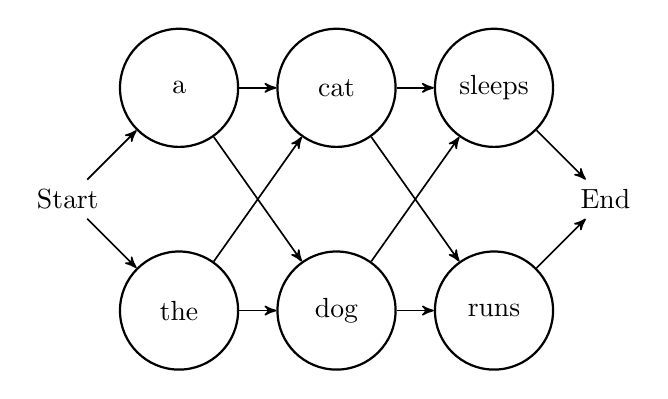
\begin{tikzpicture}[->, >=stealth', auto, semithick, node distance=2cm]
\tikzstyle{every state}=[fill=white,draw=black,thick,text=black,scale=1,minimum size=1.5cm]

\node[]         (A)                     {Start};
\node[state]    (B)[above right of=A]   {a};
\node[state]    (C)[right of=B]    {cat};
\node[state]    (D)[right of=C]   {sleeps};
\node[state]    (E)[below right of=A]   {the};
\node[state]    (F)[right of=E]   {dog};
\node[state]    (G)[right of=F]   {runs};
\node[]         (H)[above right of=G]   {End};

\path (A) edge [->]     node {}         (B);
\path (A) edge [->]     node {}         (E);

\path (B) edge [->]     node {}         (C);
\path (B) edge [->]     node {}         (F);

\path (C) edge [->]     node {}         (D);
\path (C) edge [->]     node {}         (G);

\path (D) edge [->]     node {}         (H);

\path (E) edge [->]     node {}         (C);
\path (E) edge [->]     node {}         (F);

\path (F) edge [->]     node {}         (D);
\path (F) edge [->]     node {}         (G);

\path (G) edge [->]     node {}         (H);

\end{tikzpicture}

\end{document}